\synctex=1
\documentclass[dvipdfmx,10pt, a4j]{jarticle}
%----------------------------------------------------------
%パッケージ読み込み
\usepackage{amsmath}
\usepackage{amssymb}
\usepackage{amsthm} %定理環境の拡張
\usepackage{ascmac}
\usepackage{bm}
\usepackage{cases}
\usepackage{comment} %非表示にするためのコメント
\usepackage{enumerate}
\usepackage{float} %画像をその場に表示.[h]の代わりに[H]
\usepackage{graphicx} % eps 形式の図版取り込みのため
\usepackage{mathrsfs}
\usepackage{url}
\usepackage[dvipdfmx]{hyperref}
\usepackage{color}
\usepackage{mathrsfs}
%----------------------------------------------------------

%----------------------------------------------------------
%命題関係の定義
\theoremstyle{definition}
\newtheorem{definition}{定義}[section]
\newtheorem{theorem}{定理}[section]
\newtheorem{proposition}[theorem]{命題}
\newtheorem{lemma}[theorem]{補題}
\newtheorem{col}[theorem]{系}
\newtheorem{example}{例}[section]
\newtheorem{remark}{注意}[section]
%----------------------------------------------------------

%タイトル・著者===================================================
\title{第11回 数理統計 レポート}
\author{小森 一輝}
%=================================================================

%本文開始=========================================================
\begin{document}

\maketitle

%カウンタ--------------------------------------------------
\setcounter{section}{2}
%\setcounter{subsection}{0}
%\setcounter{subsubsection}{0}
%\setcounter{theorem}{0}

%----------------------------------------------------------命題4.11
\noindent
\textbf{命題 4.11.} 共分散の性質\\
%---------------以下図
\begin{figure}[htbp]
  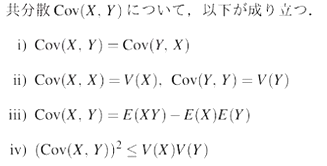
\includegraphics[width=7.0cm]{D_11/meidai/4_11.png}
\end{figure}

\begin{proof}
    iv) の証明\\
    任意の確率変数X, Y に対して, 確率変数Z, W を次の式で求める.\\
    \begin{align*}
      &Z = \frac{X-E(X)}{\sqrt{V(X)}}, \quad W = \frac{Y-E(Y)}{\sqrt{V(Y)}} \quad \to \quad
      \begin{cases}
        E(Z) = E(W) = 0\\
        V(Z) = V(W) = 1  
      \end{cases}
    \end{align*}
    \begin{align*}
      E(ZW) &= E(\frac{X-E(X)}{\sqrt{V(X)}} \cdot \frac{Y-E(Y)}{\sqrt{V(Y)}})\\
      &= \frac{E((X-E(X))(Y-E(Y)))}{\sqrt{V(X)V(Y)}}\\
      &= \frac{Cov(X, Y)}{\sqrt{V(X)V(Y)}} \leq E(Z^2)E(W^2) = 1 \qquad (\because 標準化とヘルダーの不等式)\\
      &Cov(X, Y) \leq \sqrt{V(X)V(Y)}\\
      &(Cov(X, Y))^2 \leq V(X)V(Y)\\
    \end{align*}
\end{proof}

%---------------以下補足
\begin{itembox}[l]{ヘルダーの不等式}
  \begin{align*}
    &(E(ZW))^2 \leq E(Z^2)E(W^2)\\
    &E(Z) = E(W) = 0のとき,\\
    &Cov(Z, W) \leq V(Z)V(W)\\
  \end{align*}
\end{itembox}\\

%----------------------------------------------------------命題4.12
\noindent
%---------------以下図
\begin{figure}[htbp]
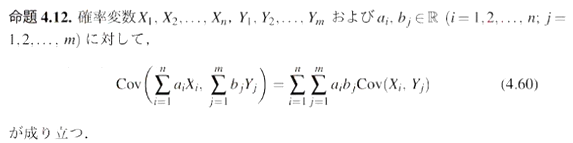
\includegraphics[width=\linewidth]{D_11/meidai/4_12.png}
\end{figure}
%---------------以下補足
\begin{itembox}[l]{補足}
  確率変数の和の共分散は, 確率変数の共分散の和になる.
\end{itembox}\\

%----------------------------------------------------------定義4.17
\noindent
\textbf{定義 4.17.} 相関係数\\
%---------------以下図
\begin{figure}[htbp]
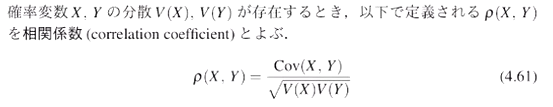
\includegraphics[width=\linewidth]{D_11/teigi/4_17.png}
\end{figure}

%----------------------------------------------------------定理4.13
\noindent
\textbf{定理 4.13.} 相関係数の性質\\
%---------------以下図
\begin{figure}[htbp]
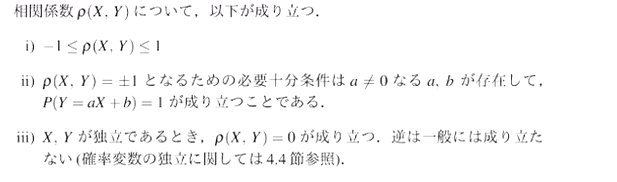
\includegraphics[width=\linewidth]{D_11/teiri/4_13.png}
\end{figure}
\begin{align*}
  &i)\\
  &(Cov(X, Y))^2 \leq V(X)V(Y) より導かれる.\\
\end{align*}
%---------------以下補足
\begin{itembox}[l]{補足}
  確率変数の\\
  $独立 \neq 無相関 \qquad 独立には確率が必要.$\\
\end{itembox}\\

\noindent
{\LARGE 4.4 確率変数の独立とその条件}\\

%----------------------------------------------------------定義4.22
\noindent
\textbf{定義 4.22.} 確率変数の独立\\
%---------------以下図
\begin{figure}[htbp]
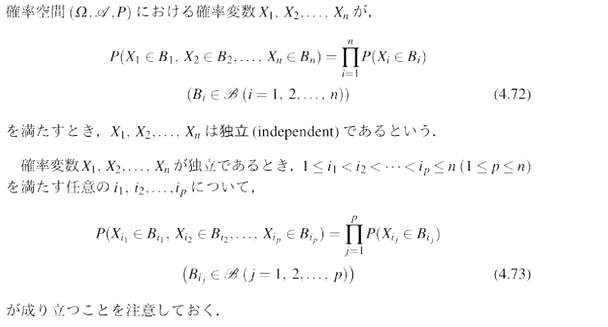
\includegraphics[width=\linewidth]{D_11/teigi/4_22.png}
\end{figure}

%---------------以下補足
\begin{itembox}[l]{補足}
  \begin{align*}
    P(X_1 \in B_1, X_2 \in B_2) = P(X_1 \in B_1)P(X_2 \in B_2)\\
  \end{align*}
  $X_1, X_2, X_3 が独立 \to X_1, X_2 は独立 \; X_1, X_3 は独立 \; X_2, X_3 は独立$\\
\end{itembox}\\

%----------------------------------------------------------定理4.18
\noindent
%---------------以下図
\begin{figure}[htbp]
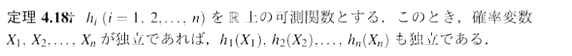
\includegraphics[width=\linewidth]{D_11/teiri/4_18.png}
\end{figure}

%---------------以下補足
\begin{itembox}[l]{補足}
  \begin{align*}
    \begin{cases}
      XとYが独立\\
      aX+b と cX+d も独立\\
      X^2 と Y^2 も独立\\
    \end{cases}
  \end{align*}
\end{itembox}\\

%----------------------------------------------------------定理4.19
\noindent
\textbf{定理 4.19.} 確率変数の独立(分布関数)\\
%---------------以下図
\begin{figure}[htbp]
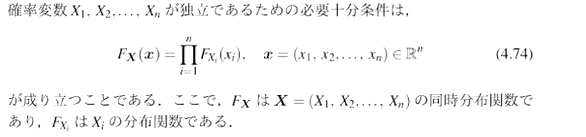
\includegraphics[width=\linewidth]{D_11/teiri/4_19.png}
\end{figure}

%----------------------------------------------------------定理4.20
\noindent
\textbf{定理 4.20.} 確率変数の独立(確率関数・確率密度関数)\\
%---------------以下図
\begin{figure}[htbp]
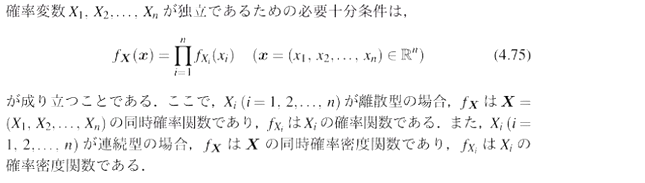
\includegraphics[width=\linewidth]{D_11/teiri/4_20.png}
\end{figure}
\begin{align*}
  &母集団 X ~ F_X \; E(X) = \mu \; V(X) = \sigma^2\\
  &独立同一の分布(iid)に従う.\\
  &X_1, X_2, \cdots , X_n - F_X\\
  &標本分布 f_X(x_1, x_2, \cdots , x_n)\\
  &= \prod_{i=1}^{n}f_X(x_i)\\
\end{align*}

%----------------------------------------------------------命題4.21
\noindent
%---------------以下図
\begin{figure}[htbp]
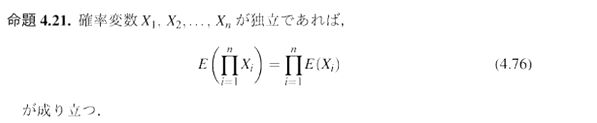
\includegraphics[width=\linewidth]{D_11/meidai/4_21.png}
\end{figure}

%----------------------------------------------------------定理4.22
\noindent
\textbf{定理 4.22.} 確率変数の独立(積率母関数)\\
%---------------以下図
\begin{figure}[htbp]
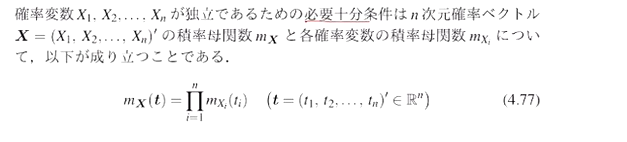
\includegraphics[width=\linewidth]{D_11/teiri/4_22.png}
\end{figure}

%----------------------------------------------------------定義4.24
\noindent
\textbf{定義 4.24.} 独立同一分布\\
%---------------以下図
\begin{figure}[htbp]
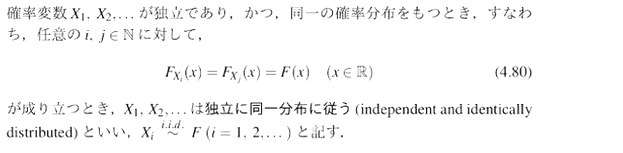
\includegraphics[width=\linewidth]{D_11/teigi/4_24.png}
\end{figure}\\
※無作為標本とiidは必要十分条件\\

\newpage
%----------------------------------------------------------定理4.25
\noindent
\textbf{定理 4.25.} 畳み込み\\
%---------------以下図
\begin{figure}[htbp]
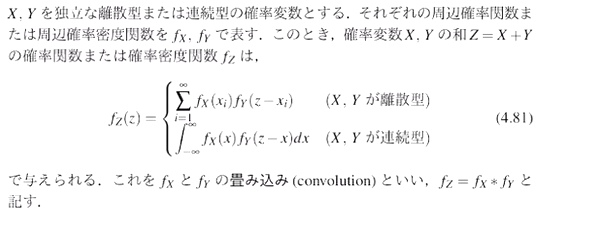
\includegraphics[width=\linewidth]{D_11/teiri/4_25.png}
\end{figure}
%---------------以下補足
\begin{itembox}[l]{補足}
  \begin{align*}
    f_Z(Z) =
    \begin{cases}
      \sum_{i=1}^{\infty}f_{X, Y}(x_i, Z-x_i) = \sum f_X(x_i) f_Y(z-x_i)\\
      \int_{-\infty}^{\infty}f_{X, Y}(x_i, Z-x_i) = \int_{-\infty}^{\infty}f_X(x_i) f_Y(z-x_i)
    \end{cases}
  \end{align*}
\end{itembox}\\

%----------------------------------------------------------定理4.26
\noindent
\textbf{定理 4.26.} 独立な連続型確率変数の積と商の分布\\
%---------------以下図
\begin{figure}[htbp]
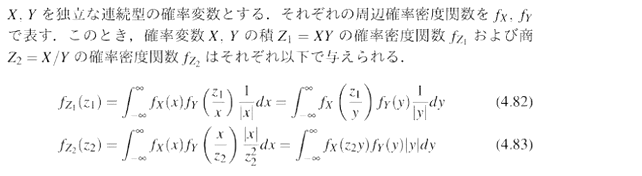
\includegraphics[width=\linewidth]{D_11/teiri/4_26.png}
\end{figure}\\
定理\\
$確率変数 X_i が独立のとき,$\\
\begin{align*}
  &Z = \sum_{i=1}^{n}X_iの積率母関数m_Z(t)は以下で与えられえる.\\
  &m_Z(t) = \prod_{i=1}^{n}m_{X_i}(t)\\
  &和の積率母関数は, 積率母関数の積\\
\end{align*}
\begin{proof}
  \begin{align*}
    m_Z(t) &= E(e^{t(X_1 + X_2 + \cdots + X_n)})\\
    &=\prod_{i=1}^{n}E(X^{tX_i})\\
    &=\prod_{i=1}^{n}m_{X_i}(t)\\
  \end{align*}
\end{proof}

\noindent
{\LARGE 4.5 条件付き期待値}\\
%----------------------------------------------------------定義4.26
\noindent
\textbf{定義 4.26.} 条件付き期待値\\
%---------------以下図
\begin{figure}[htbp]
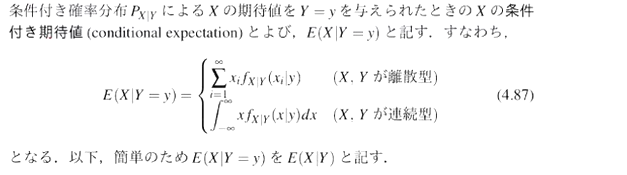
\includegraphics[width=\linewidth]{D_11/teigi/4_26.png}
\end{figure}

%----------------------------------------------------------定義4.27
\noindent
%---------------以下図
\begin{figure}[htbp]
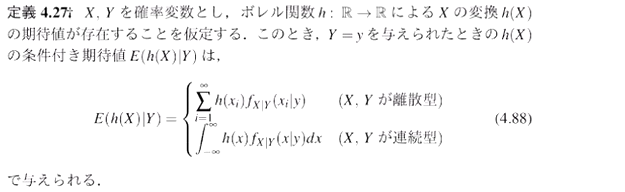
\includegraphics[width=\linewidth]{D_11/teigi/4_27.png}
\end{figure}

%----------------------------------------------------------命題4.28
\noindent
\textbf{命題 4.28.} 条件付き期待値の性質\\
%---------------以下図
\begin{figure}[htbp]
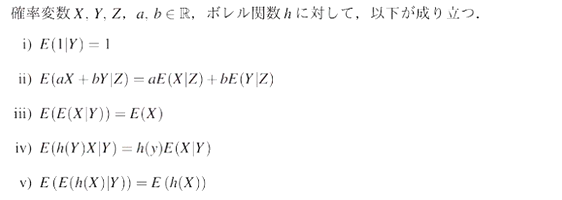
\includegraphics[width=\linewidth]{D_11/meidai/4_28.png}
\end{figure}
\begin{enumerate}[i)]
  \item $E(1|Y) = \int_{-\infty}^{\infty} 1 \cdot f_{X|Y}dx = 1$\\
  \item $E(aX + bY | Z)$
  \begin{align*}
    E(aX + bY | Z) &= \int_{-\infty}^{\infty}\int_{-\infty}^{\infty}f_{X|Y}(x, y|z)dxdy\\
    &= a \int\int x f_{X, Y|Z}(x, y|z)dxdy + b \int\int y f_{X, Y|Z}(x, y|z)dxdy\\
    &= a \int x\int f_{X, Y|Z}(x, y|z)dxdy + b \int y\int f_{X, Y|Z}(x, y|z)dxdy\\
    &= a \int x f_{X|Z}(x|z)dxdy + b \int y f_{Y|Z}(y|z)dy\\
    &= a E(X|Z) + bE(Y|Z)\\
  \end{align*}
  \item $E(E(X|Y)) = \int_{-\infty}^{\infty}$
  \begin{align*}
    E(E(X|Y)) &= \int_{-\infty}^{\infty}E(X|Y)f_Y(y)dy\\
    &= \int (\int x f_{X|Y}(x|y)dx)f_Y(y)dy\\
    &= \int \int x f_Y(y)f_{X|Y}(x|y)dxdy\\
    &= \int \int x f_X(x, y(x|y)dxdy = \int x (\int f_X(x, y)dy)dx\\
    &= \int x f(x)dx = E(X)\\
  \end{align*}
  \item $E(h(Y)X|Y)$\\
  \begin{align*}
    E(h(Y)X|Y) &= h(y)\int x f_{X|Y}(x|y)dx\\
    &= h(y)E(X|Y)\\
  \end{align*}
  \item iii)と同様\\
\end{enumerate}

%----------------------------------------------------------定義4.29
\noindent
\textbf{定義 4.29.} 条件付き分散\\
%---------------以下図
\begin{figure}[htbp]
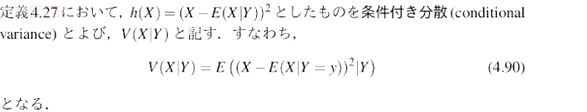
\includegraphics[width=\linewidth]{D_11/teigi/4_29.png}
\end{figure}

%----------------------------------------------------------命題4.29
\noindent
\textbf{命題 4.29.} 条件付き分散の性質\\
%---------------以下図
\begin{figure}[htbp]
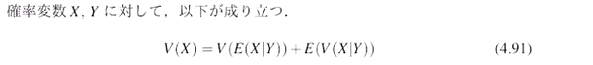
\includegraphics[width=\linewidth]{D_11/meidai/4_29.png}
\end{figure}
\begin{proof}
  \begin{align*}
    V(X|Y) = E(X^2|Y)-(E(X|Y))^2\\
    V(X|Y) &= E((X - E(X|Y))^2)\\
    &= E(X^2 - 2XE(X|Y) + (E(X|Y))^2)\\
    &= E(X^2|Y)-2(E(X|Y))^2 + (E(X|Y))^2\\
    &= E(X^2|Y) - (E(X|Y))^2\\
  \end{align*}
  \begin{align*}
    V(E(X|Y)) &= E((E(X|Y))^2 - (E(E(X|Y))^2))\\
    &= E_Y((E(X|Y))^2)-(E(X))^2\\
  \end{align*}
  \begin{align*}
    E(V(X|Y)) &= E_{Y}(E((X^2|Y)-E(X|Y))^2)\\
    &= E(X^2) - E((E(X|Y))^2)\\
    よって, V(E(X|Y) + E(V(X|Y))) = E(X^2)-(E(X))^2 = V(X)\\
  \end{align*}
\end{proof}
%---------------以下補足
\begin{itembox}[l]{補足}
  $V(X|Y) = E(X^2|Y)-(E(X|Y))^2$\\
\end{itembox}\\

\end{document}
%本文ここまで=========================================================